\section{Zusammenstellung Signalformen}
\begin{table}[htdp]
\begin{center}
\begin{tabular}{|c|c|c|c|c|p{6cm}|}
\hline
\textbf{Signal} & \textbf{Funktion} & \textbf{$X_0$} & \textbf{$X^2$} & \textbf{var(X)} & \textbf{Hinweise} \\

\hline
\parbox[c][2.1cm]{3.5cm}{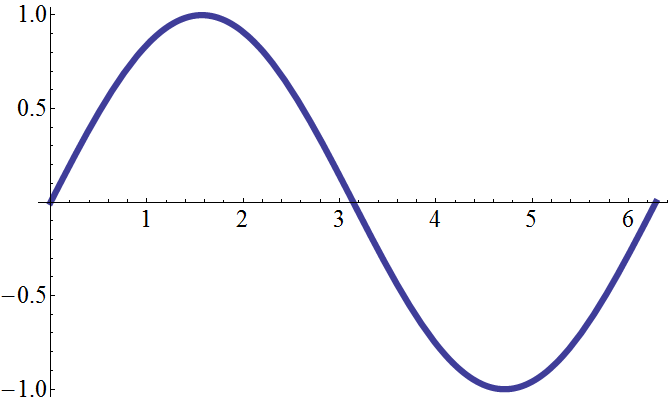
\includegraphics[height=2cm]{./bilder/Signale/Sinus.png}} &
$A\cdot\sin(t)$  & $0$ &
$\frac{A^2}{2}$ & $\frac{A^2}{2}$
&  \\

\hline
\parbox[c][2.1cm]{3.5cm}{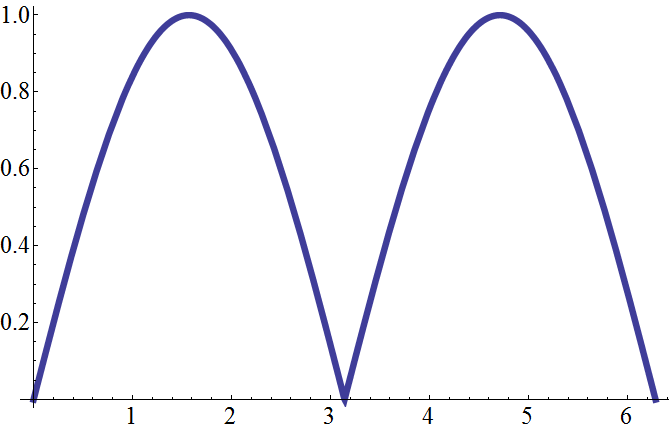
\includegraphics[height=2cm]{./bilder/Signale/AbsSinus.png}} &
$A\cdot|\sin(t)|$  &
$\frac{2A}{\pi}$ & $\frac{A^2}{2}$ & $\frac{A^2}{2}-\frac{4A^2}{\pi^2}$
& \\

\hline
\parbox[c][2.1cm]{3.5cm}{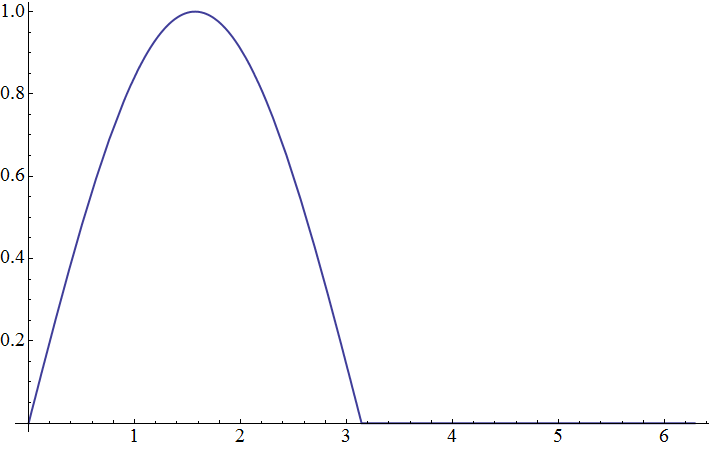
\includegraphics[height=2cm]{./bilder/Signale/Sinus_ersteWelle.png}} &
$\begin{cases} A\cdot\sin (t) & 0<t<\pi  \\ 0 & \text{True}\end{cases}$ & $\frac{A}{\pi}$ &
$\frac{A^2}{4}$ & $\frac{A^2}{4}-\frac{A^2}{\pi^2}$
& \\

\hline
\parbox[c][2.1cm]{3.5cm}{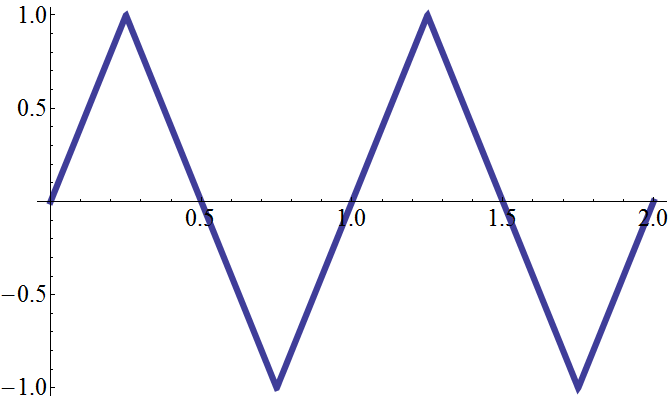
\includegraphics[height=2cm]{./bilder/Signale/Dreieck2.png}} &
$A\cdot\Lambda(t)$
& $0$ & $\frac{A^2}{3}$ &
$\frac{A^2}{3}$
& Form des $\Lambda$ egal! \\

\hline
\parbox[c][2.1cm]{3.5cm}{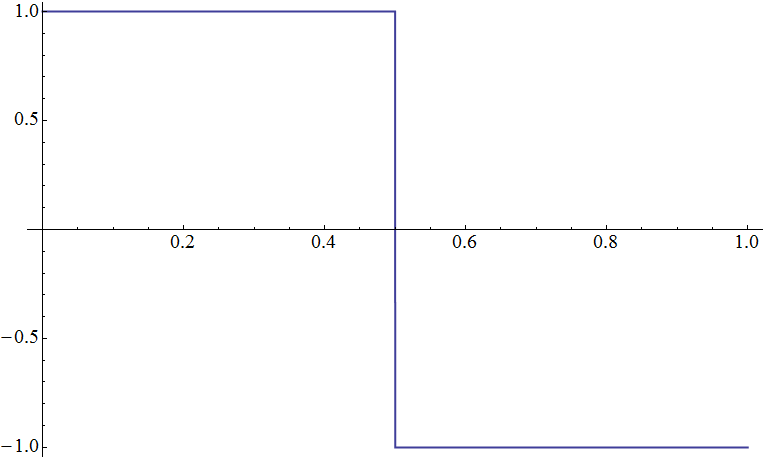
\includegraphics[height=2cm]{./bilder/Signale/UnitStep.png}} &
$A\cdot\prod(t)$
& $0$ & $A^2$ & $A^2$
& \\

\hline
\parbox[c][2.1cm]{3.5cm}{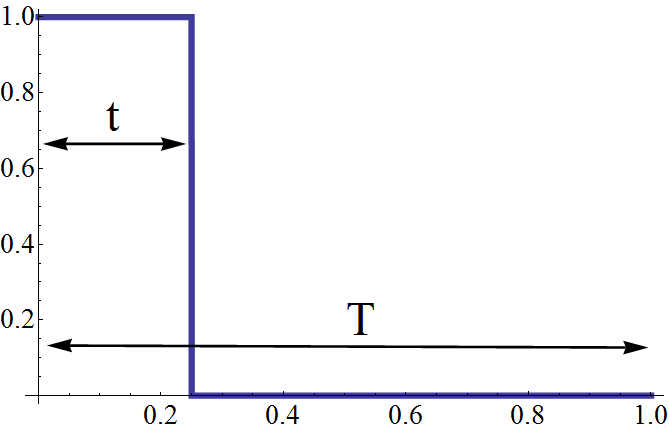
\includegraphics[height=2cm]{./bilder/Signale/StepAt_t.png}} &
$\begin{cases} A & 0<x<t \\ 0 & \text{True}\end{cases}$ 
& $A\frac{t}{T}$ &
$A^2\frac{t}{T}$ & $\frac{A^2t}{T}-\frac{A^2t^2}{T^2}$
& \\

\hline
\end{tabular}
\end{center}
\end{table}

\textbf{Allgemeine Hinweise:}
\begin{itemize}
  \item Wenn das Signal nicht symetrisch zur x-Achse ist, lässt sich der Quadratische Mittelwert einfacher über die
  Varianz berechnen. ($X^2 = X_0^2 + Var(x)$)
  \item Mittelwert \& Quadratischer Mittelwert lassen sich bei zusammengesetzten Funktionen durch zusammenzählen der
  einzelnen Stücke berechnen. Achtung: Einzelstücke richtig gewichten!
\end{itemize}
